%%%%%%%%%%%%%%%%%%%%%%%%%%%%%%%%%%%%%%%%%%%%%%%%%%%%%%%%%%%%%%%%%%%%%%%%%%%%%%%%
%2345678901234567890123456789012345678901234567890123456789012345678901234567890
%        1         2         3         4         5         6         7         8

\documentclass[letterpaper, 10 pt, conference]{ieeeconf}  % Comment this line out if you need a4paper

%\documentclass[a4paper, 10pt, conference]{ieeeconf}      % Use this line for a4 paper

\IEEEoverridecommandlockouts                              % This command is only needed if 
                                                          % you want to use the \thanks command

\overrideIEEEmargins                                      % Needed to meet printer requirements.

%In case you encounter the following error:
%Error 1010 The PDF file may be corrupt (unable to open PDF file) OR
%Error 1000 An error occurred while parsing a contents stream. Unable to analyze the PDF file.
%This is a known problem with pdfLaTeX conversion filter. The file cannot be opened with acrobat reader
%Please use one of the alternatives below to circumvent this error by uncommenting one or the other
%\pdfobjcompresslevel=0
%\pdfminorversion=4

% See the \addtolength command later in the file to balance the column lengths
% on the last page of the document

\usepackage{cleveref}
\crefname{figure}{fig}{figs}
\usepackage{epsfig}
\usepackage{float}
\usepackage{threeparttable}
\usepackage{subfigure}

% The following packages can be found on http:\\www.ctan.org
%\usepackage{graphics} % for pdf, bitmapped graphics files
%\usepackage{epsfig} % for postscript graphics files
%\usepackage{mathptmx} % assumes new font selection scheme installed
%\usepackage{times} % assumes new font selection scheme installed
%\usepackage{amsmath} % assumes amsmath package installed
%\usepackage{amssymb}  % assumes amsmath package installed

\title{\LARGE \bf
Data-Efficient and Hardware  Decentralized Visual {SLAM}
}


\author{Jincheng Yu$^{1}$ and Feng Gao$^{1}$ % <-this % stops a space
% \thanks{*This work was not supported by any organization} % <-this % stops a space
\thanks{$^{1}$Electronic Engineering Department,
        Tsinghua University, Beijing, China
        {\tt\small yjc16@mails.tsinghua.edu.cn}}%
% \thanks{$^{2}$Bernard D. Researcheris with the Department of Electrical Engineering, Wright State University,
%         Dayton, OH 45435, USA
%         {\tt\small b.d.researcher@ieee.org}}%
}


\begin{document}

\maketitle
\thispagestyle{empty}
\pagestyle{empty}


%%%%%%%%%%%%%%%%%%%%%%%%%%%%%%%%%%%%%%%%%%%%%%%%%%%%%%%%%%%%%%%%%%%%%%%%%%%%%%%%
\begin{abstract}
Decentralized visual simultaneous localization and mapping (DSLAM) can share locations and environmental information between robots, which is an essential task for many multi-robot applications. For \textit{"robot"}, the Visual Odometry (VO) is a basic component to estimate the 6-DoF absolute pose, and for \textit{"multi"}, Decentralized Place Recognition (DPR) is a fundamental element to produce candidate place matches.
%Due to the advantages of Convolutional Neural Network(CNN) on image processing tasks, CNN-based VO and DPR have achieved significant improvements in performance., such as Depth-VO-Feat\cite{Zhan:2018e92} and NetVLAD\cite{Arandjelovic:2017997}. However, previous works concentrate on the accuracy of the CNNs, yet consider little about the deployment CNNs on the embedded system.
Although some CNN-based VO and DPR methods have made significant progress in performance compared to feature-based methods, such as Depth-VO-Feat \cite{Zhan:2018e92} and NetVLAD \cite{Arandjelovic:2017997}, they focus primarily  on the accuracy of CNNs, yet consider little about the deployment of CNNs on embedded systems.

Since the embedded system usually only supports fixed-point CNN, we propose a pose-sensitive fixed-point finetune method for the CNN-based monocular VO, and accelerate the per-frame VO from 230ms to 10ms with similar accuracy. In addition, empirical experiments show that the frequency of DPR has a large impact on the final result of DSLAM. So we propose a cross-component pipeline scheduling method to increase the computational speed of NetVLAD from once every 12 frames to once every 8 frames, and further improve the final accuracy of DSLAM.
% We find the tranditional average trajectory error (ATE) can not indicate the performance of trajectory merging in DSLAM, so we propose a new indicator called loop-closure recall (LCR) to evaluate the performance of trajectory merging.

% With the gradual improvement of the single-agent capabilities, it is possible to build up the multi-agent collaborative intelligence system.
% Distributed simultaneous localization and mapping (DSLAM) can share location and environmental information between robots and is the basis for many multi-agent applications.
% With the development of algorithms and computing platforms in recent years, convolutional neural network (CNN) has been widely used in SLAM systems, especially in visual-based SLAM systems.
% CNN can directly predict the pose with the absolute scale from two successive monocular frames, which can be easy to deploy on real robots and can make SLAM more robust in scenarios with pure rotations. Further, with CNN's versatility, it is easy to use the same network structure for many other tasks rather than depth or pose estimation, such as object detection and semantic segmentation.
% Finally, CNN's computational structure is uniform and can be individually optimized when resources are limited on embedded systems.

% In this work, we aim to build a fully CNN-based hardware-software co-design monocular DSLAM system. There are two keys components in DSLAM system: 1) Visual Odometry (VO) and 2) Place Recognition. We use fixed-point fine tune method to enhance the accuracy of CNN-based monocular VO and make it possible for acceleration on the Xilinx DPU accelerator. The same DPU also supports the place recognition component. We also propose a pipeline scheduling method to make full use of the DPU. To the best of our knowledge, this work is the first to implement all components of monocular DSLAM with CNN. We use the Xilinx ZU9 embedded MPSoC and the DPU IP core to validate the proposed DSLAM framework on the public dataset.
\end{abstract}

\section{Introduction}
\label{sec:introdutction}
In recent years, the capabilities of a single agent have been significantly improved. To further expand the capabilities of intelligent robots, using several robots can accelerate many tasks, such as localization, exploration, and mapping.
Decentralized visual simultaneous localization and
mapping (DSLAM) can share location and environmental information between robots and is the essential task for many multi-robot applications. \cite{Cieslewski:20187ee} concludes the basic procedure as \cref{fig:all}

\begin{figure}[h]  
    \centering  
    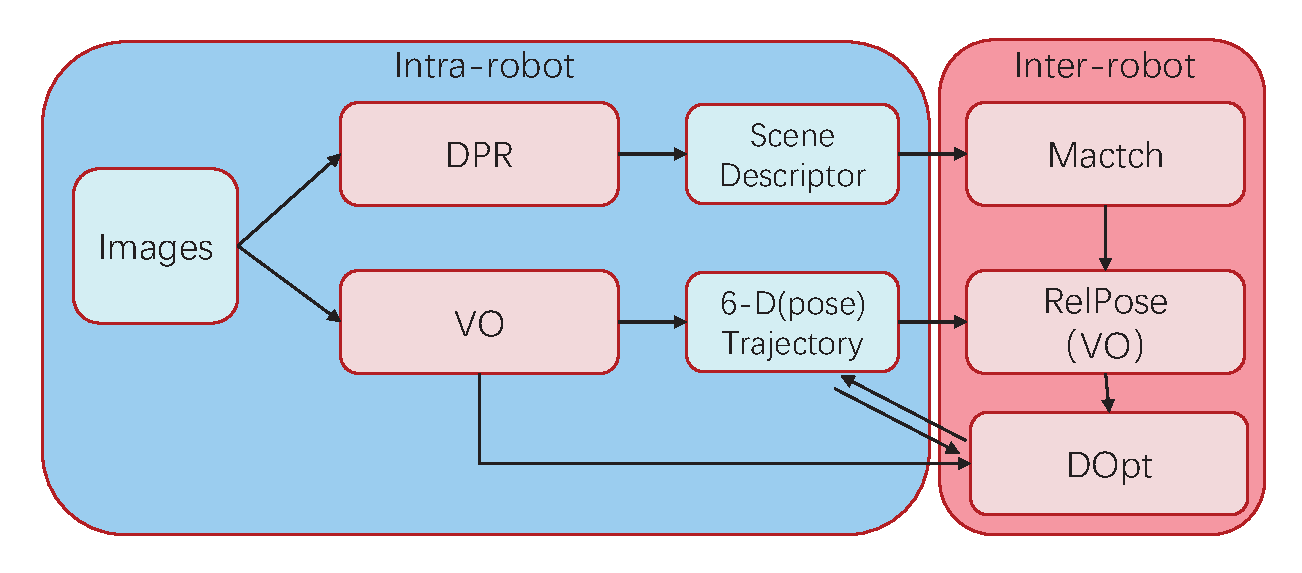
\includegraphics[width=0.75\linewidth]{fig/all.eps}
    \caption{DSLAM framework\cite{Cieslewski:20187ee}. \textbf{VO} is used to calculate the intra-robot 6-D absolute pose from the input frames. \textbf{DPR} produces a compact image representation that communicate among robots. \textbf{Match} stage finds out candidate inter-robot place recognition matches.  \textbf{RelPose} requires data from the matched robots and establishes relative poses between the robots trajectories. \textbf{DOpt} obtains the trajectories, intra-robot pose measurements from VO and inter-robot relative poses from RelPose, and updates the trajectories.}
    \label{fig:all}
\end{figure}

There are five components: DPR, VO, Match, RelPose and DOpt. DPR and VO are intra-robot operations, and require high computation resources on embedded system. Match, RelPose and DOpt are inter-robot operations, and consume most of the communication of DSLAM sytem. The RelPose components can and should depend the VO components since it can benefit from re-using the data and computation resources of VO.

The previous work \cite{Cieslewski:20187ee} uses ORB feature-point based method to estimate the trajectory from the sequence of the stereo camera, and use NetVLAD \cite{Arandjelovic:2017997} to do place recognition. These two algorithms both consume a large amount of computation and storage, and pose a great challenge to DSLAM on the embedded system. The DSLAM frame in \cite{Cieslewski:20187ee} is illustrated in \cref{fig:all_pre}.


\begin{figure*}[thb]
    \begin{minipage}[t]{0.5\linewidth}  
    \centering
    \subfigure[DSLAM in \cite{Cieslewski:20187ee}] {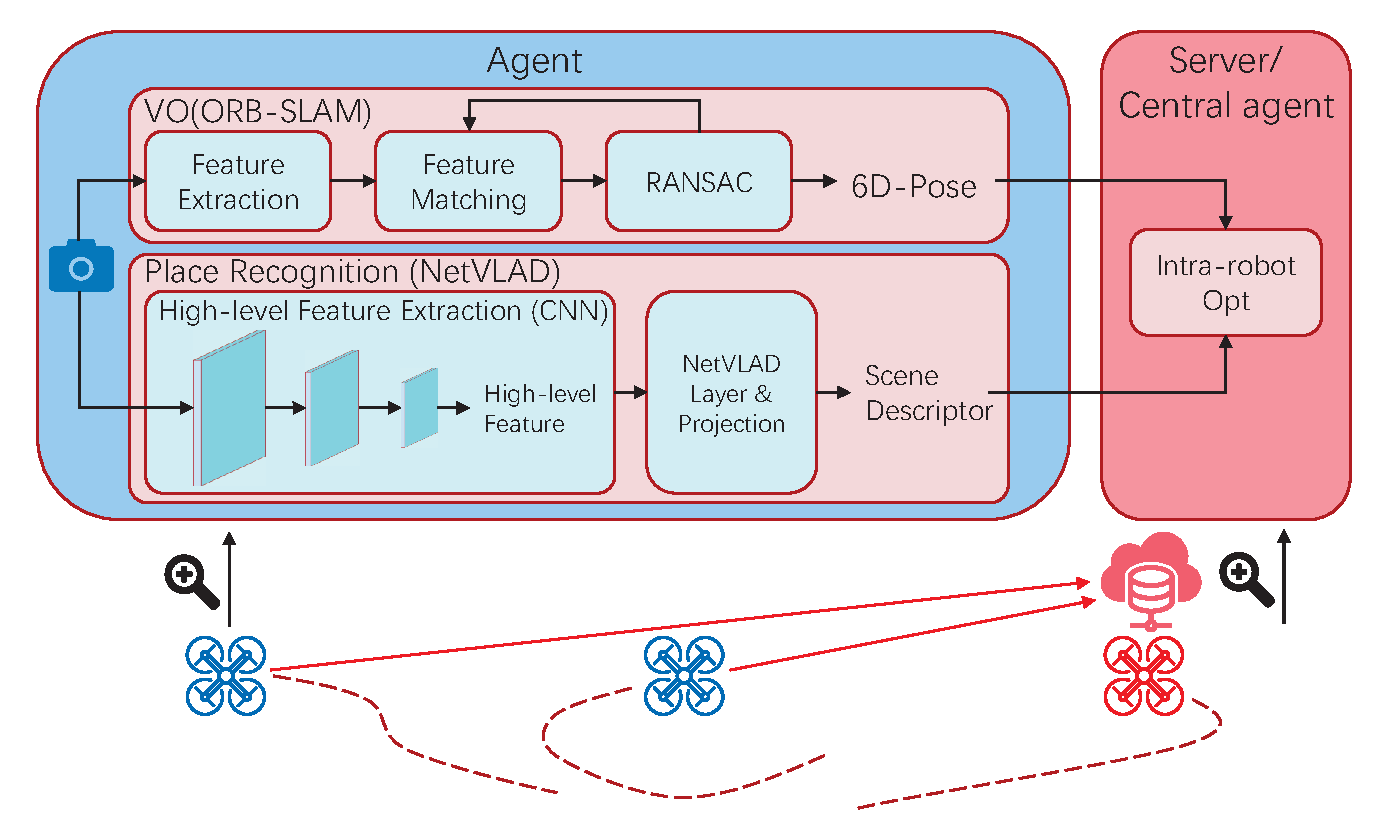
\includegraphics[width=0.8\textwidth]{fig/overview_pre.eps}\label{fig:all_pre}}
    \end{minipage}
    \begin{minipage}[t]{0.5\linewidth}  
    \centering  
    \subfigure[Our hardware-software co-design DSLAM.] {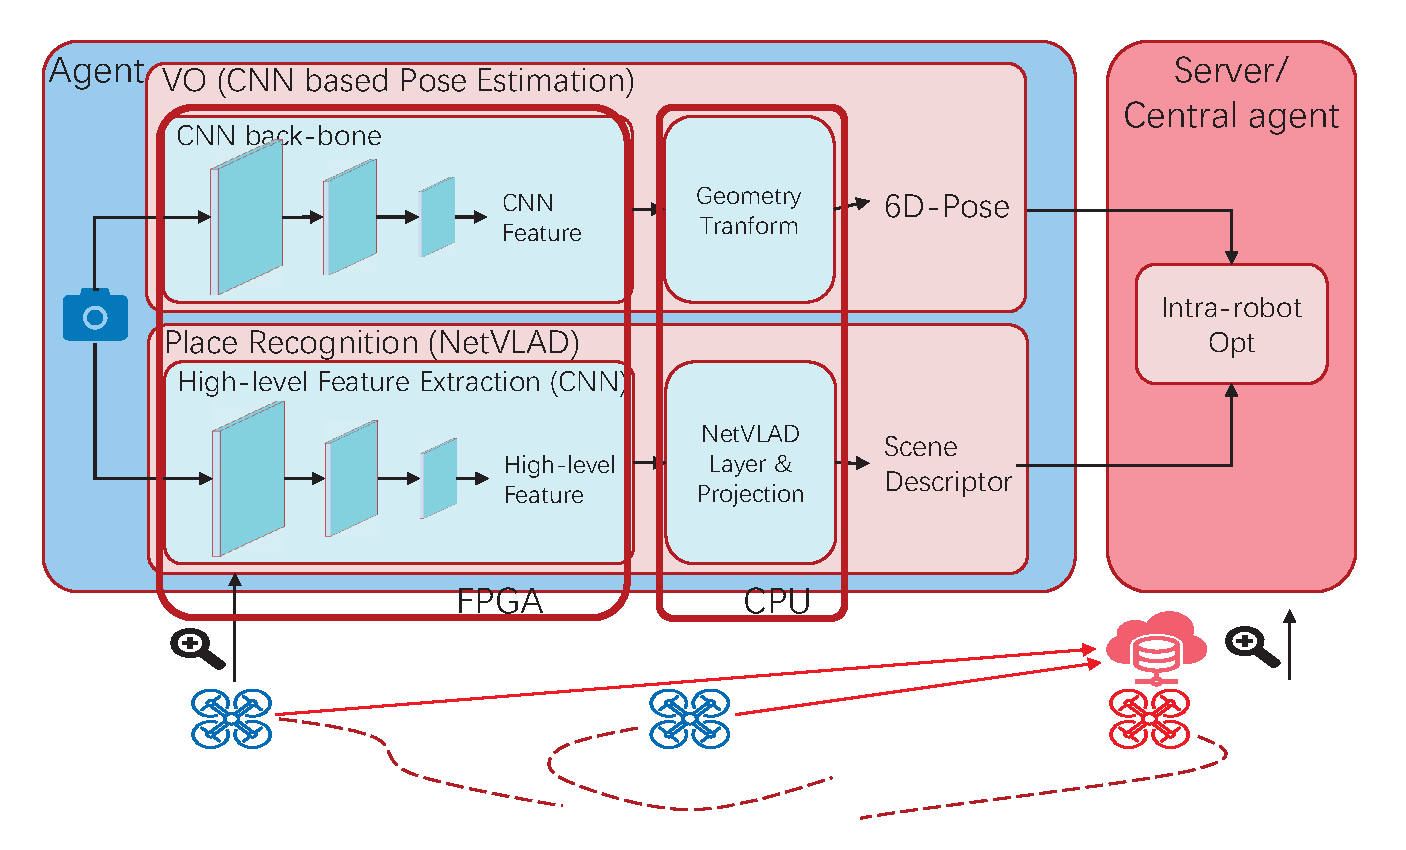
\includegraphics[width=0.8\linewidth]{fig/overview_us.eps}\label{fig:all_us}} 
    \end{minipage}
    \caption{???
    % Overview of the DSLAM in \cite{Cieslewski:20187ee} and our hardware-software co-design DSLAM. Each agent (blue drones) will send the result of 6-D pose estimation and scene descriptor to a server or a central agent (red server or drone in figure) to do inter-robot place recognition and optimization. We use CNN instead of feature points to do pose estimation so that we can use CNN accelerator to speed up the whole process.
    }
\label{fig:overview}
\end{figure*}

Monocular systems are much easier to deploy than binocular systems. The transitional monocular feature point based VO should use complex depth reconstruction methods to compute the absolute scale of the pose scale\cite{pizzoli2014remode}, leading to speed-down. With the development of CNN, we can reconstruct the depth and pose with the absolute scale from the monocular camera directly, making monocular VO more robust and efficient\cite{Zhan:2018e92}. ecent advances in deep learning and the availability of large labelled visual datasets have significantly improved the accuracy of place recognition, such as NetVLAD\cite{Arandjelovic:2017997}. However, previous works concentrate on the accuracy of the CNNs, yet consider little about the deployment CNNs on the embedded system.

Though DSLAM system can benefit from the development of CNN, the fully CNN-based DSLAM system faces some key issues: 1) The embedded system usually support fixed-point CNN. 2) The speed will decline in the embedded system when running several CNN models simultaneously, the speed-down of DPR will lead to the decline of the final DSLAM accuracy. Therefore, we build up a CNN-based monocular DSLAM system on embedded FPGA platform, with following contributions:

\begin{itemize}
\item To the best of our knowledge, this work is the first to implement all components of monocular DSLAM with CNN.
% We adopt Depth-VO-Feat \cite{Zhan:2018e92} in DSLAM system to estimate the pose from the input monocular camera. We use the same method of NetVLAD in  \cite{Cieslewski:20187ee} to do place recognition. 
We deploy the system on Xilinx Zynq MPSoC hardware platform with DPU \cite{Tech:2019360}, which is an embedded CNN accelerator. The proposed DSLAM framework is illustrated in \cref{fig:all_us}.
\item As the embedded system usually support fixed-point CNN, we propose a pose-sensitive fixed-point fine-tune method to make the feature extraction layers fixed-point and remain the pose prediction layers floating-point, reaching the same accuracy with the original floating-point VO network. We schedule the fixed-point layers on DPU and the floating-point layers on CPU, so that we can accelerate the VO to 10ms.
\item The frequency of the NetVLAD influences the final result of DSLAM. We propose a cross-components scheduling method to scheduling the computation flow across VO and DPR, and pipeline the computation across the PL and PS of MPSoC to make full use of the embedded platform. We calculate the NetVLAD every 4 input frames from every 6 frames, improving the final accuracy of DSLAM. 
We also propose a new indicator called loop-closure recall (LCR), which indicates the remaining rate of loop-closure after trajectory merging, to evaluate the performance of trajectory merging.
\end{itemize}

The output result of DSLAM with different NetVLAD frequency is illustrated in \cref{fig:dslamresult}. The tranditional average trajectory error (ATE) can not indicate the performance of trajectory merging in DSLAM. 

\begin{figure}[thb]
    \begin{minipage}[t]{0.475\linewidth}  
    \centering
    \subfigure[NetVLAD/8 frames. \protect\          ATE=0.9] {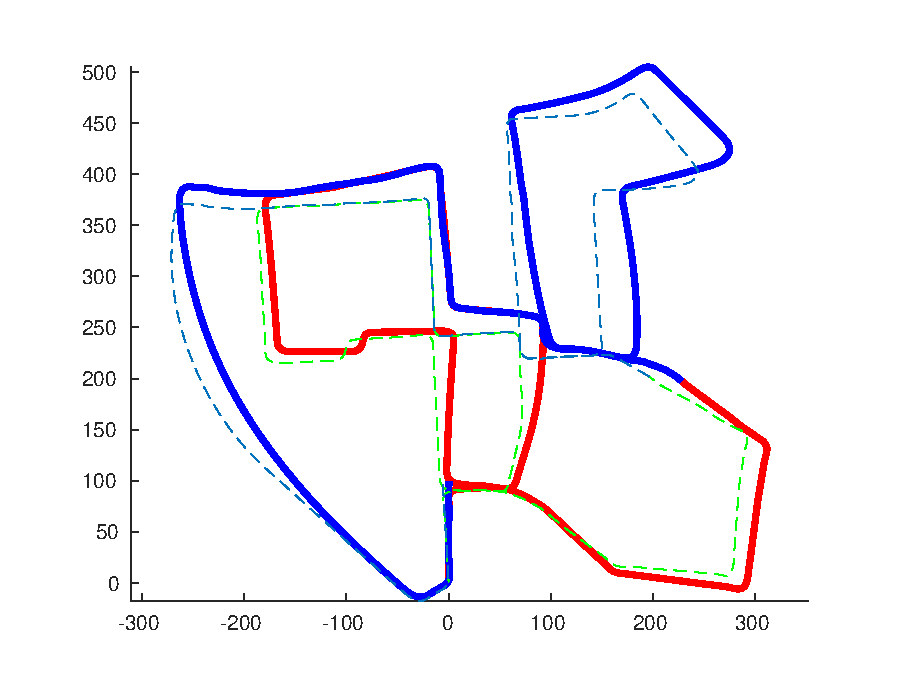
\includegraphics[width=1\linewidth]{fig/8netvlad.eps}\label{fig:8netvlad}}
    \end{minipage}
    \begin{minipage}[t]{0.475\linewidth}  
    \centering  
    \subfigure[NetVLAD/12 frames. \protect\ ATE=0.9] {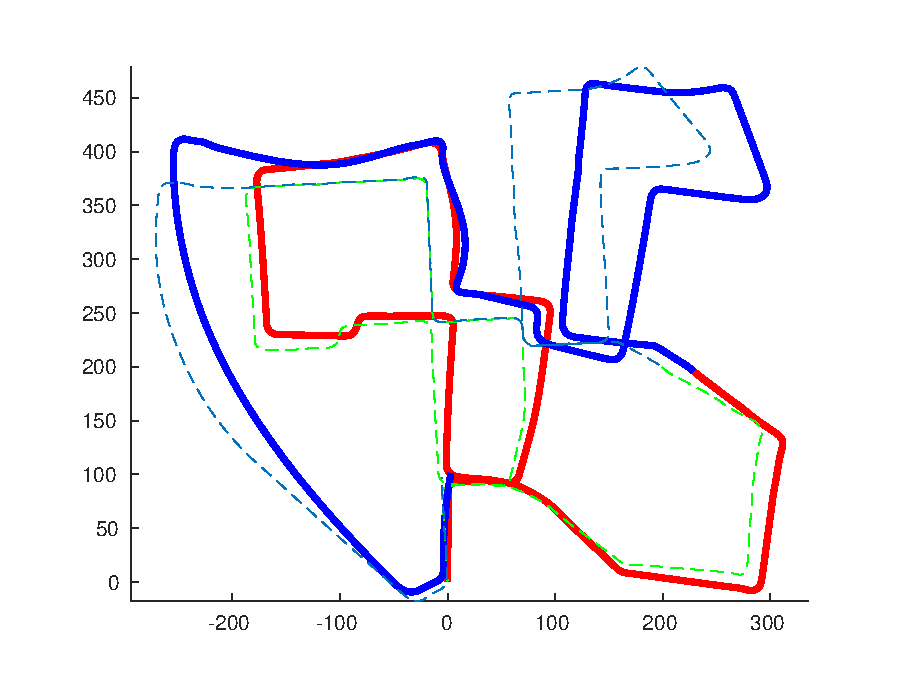
\includegraphics[width=1\linewidth]{fig/12netvlad.eps}\label{fig:12netvlad}} 
    \end{minipage}
    \caption{The result of DSLAM. \Cref{fig:8netvlad} do NetVLAD every 8 frames, and the frame con
    }
\label{fig:dslamresult}
\end{figure}



% The rest part of this article is orgnized as follows. \Cref{sec:background} will give the basic idea of CNN based methods and the hardware architecture of embedded platform, Xilinx Zynq MPSoC. \Cref{sec:hardsoft} will detail the implementation of our pose-sensitive fixed-point fine-tune method and the cross-components scheduling method. The experiment results will be given in \Cref{sec:experiment}. \Cref{sec:conclusion} will conclude this paper.

\section{Background}
\label{sec:background}
\subsection{CNN based methods in DSLAM}
As described before, there are two essential components on each agent: 1) Visual Odometry (VO) and 2) Place Recognition.

\subsubsection{Visual Odometry (VO)}

Visual odometry estimation is the task to infer ego-motion from a sequence of images and is an essential component in the SLAM system. Some feature-based SLAM systems have enjoyed great success, like ORB-SLAM\cite{DBLP:journals/trob/Mur-ArtalMT15} and ORB-SLAM2\cite{Mur-Artal:2017281}. Recently, several studies have shown that these feature-based SLAM systems require high computing resources. Fang et al.\cite{Fang2017FPGAbasedOF} shows that the feature extraction stage is the most computation-intensive, consuming over 50\% of the CPU resources.

As FPGA is one of the most promising platforms as the accelerator for VO, the SLAM system on FPGA has become a hot research topic. However, FPGA-accelerated feature extraction still consumes a lot of time and computing resources, which cannot be deployed simultaneously with an FPGA-accelerated neural network.

\subsubsection{Place Recognition}

The goal of place recognition is to calculate a given frame into a limited set of places. Each place can be encoded as a concise code which can be easy transferred with low communication cost. Traditional place recognition method usually translate the input frame as the aggregation of handcrafted feature point and local descriptors, like SIFT \cite{Lowe:2004e6e} or ORB \cite{Mur-Artal:2017281}, using vectorization techniques like bag-of-words (BoW) \cite{Galvez-Lopez:2012c94} or vector of locally aggregated descriptors(VLAD) \cite{Jegou:2010f45}.

Recent advances in the deep learning and the convolution neural network (CNN) enable powerful end-to-end mode for place recognition \cite{Noh:2017d0b, Arandjelovic:2017997}, and the NetVLAD method is one of the most accurate methods based on CNN. The NetVLAD algorithm based on VGG-16 model \cite{Simonyan:20143be} consumes more than $80G$ operations for a single $300 \times 300$ input image (each operation means addition or  multiplication). It is very challenging to deploy the NetVLAD on a traditional embedded hardware platform.

\subsection{Hardware architecture of Zync MPSoC}
The Xilinx Zync MPSoC is a chip with ARM cores and FPGA fabric. The system is illustrated in \cref{fig:plps}. The ARM cores with an embedded Linux operation system are called Processing System (PS). The FPGA fabric is called Programmable Logic (PL). The peripherals like camera and communication unit (WiFi or others) are accessible with PS. The high-bandwidth on-chip AXI interface is used to communicate between PS and PL. PS and PL can also share the DDR to transfer a large volume of data such as each frame of the camera.
Deephi CNN accelerator, which is called DPU \cite{Tech:2019360}, is one of the state-of-the-art accelerators and is famous for high energy efficiency on various CNN structure. We deploy the accelerator on the PL side of Zynq SoC with the help of DPU.

\begin{figure}[t]  
    \centering  
    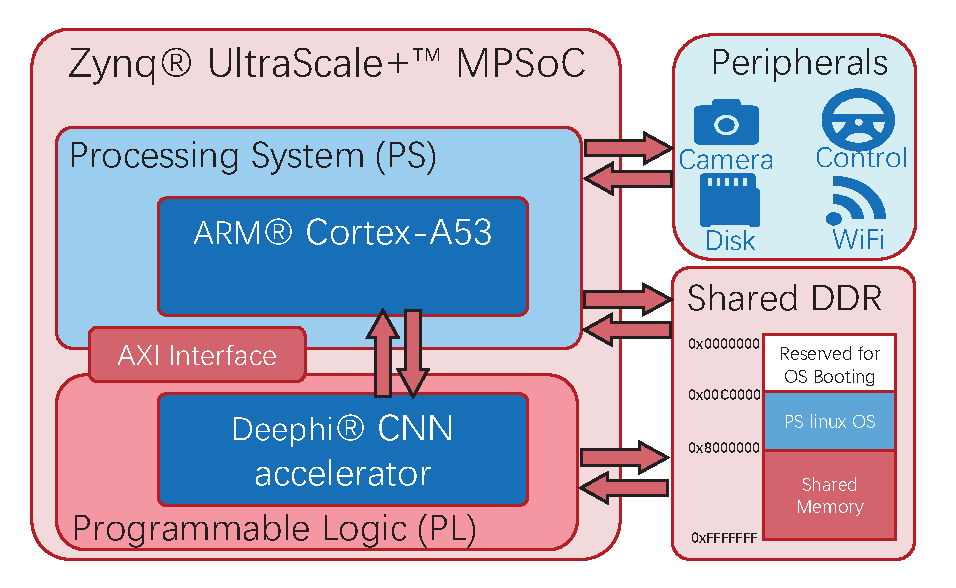
\includegraphics[width=0.95\linewidth]{fig/plps.eps}
    \caption{Hardware architecture of Zynq SoC}
    \label{fig:plps}
\end{figure}

Though FPGA can significantly improve the performance and energy efficiency of CNN inference, FPGA cannot efficiently calculate the floating-point number and requires fixed-point parameters and intermediate data in CNN.

\subsection{Motivation}
Though previous work \cite{Cieslewski:20187ee} proposes data-efficient DSLAM system, it is difficult to implement the two essential components, VO and place recognition simultaneously on a communication-limited and energy-constrained embedded hardware platform on a real robot. We propose this hardware-software co-design DSLAM system to use Xilinx Zynq MPSoC and Deephi DPU to execute these two components on the real system.




\section{Hardware-Software Co-design DSLAM}
\label{sec:hardsoft}
Our hardware-software co-design DSLAM system contains two essential improvements in the pose estimation and place recognition tasks. As illustrate in \cref{fig:all_us}, both of these two components are divided into two stages: $1)$ CNN front end to extract features which is deployed to the DPU on PL and $2)$ Algebraic operations to present final results which are deployed on the PS ARM cores. To make full use of the Zynq MPSoC, we optimize the data follow for both of these components.

\begin{figure}[t]  
    \centering  
    {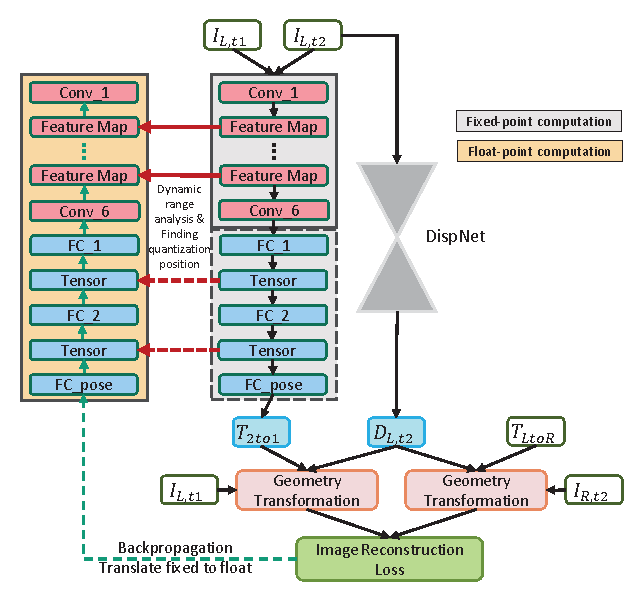
\includegraphics[width=0.8\linewidth]{fig/depth_vo_feat.eps}\label{fig:dvo}}
    \caption{Illustration of training framework for visual odometry, where $T_{LtoR}$ is the relative camera pose transformations between left and right views. To speed up the inference, we attepmt different quantization strategies to fixed-finetune the network for VO with fixed-point feed forwarding and floating-point backpropagation.}
\end{figure}

\subsection{Pose Estimation}
We adopt Depth-VO-Feat \cite{Zhan:2018e92} in DSLAM system to estimate the pose from the input monocular camera. Monocular visual SLAM is a key issue in the field of robotics, while there are two challenging problems: $1)$ it is difficult and expensive to obtain accurate labeled data, $2)$ the methods that use monocular sequences in training always suffer from the scale-ambiguity problem, i.e., the actual scale of translations is missing, and only the direction is learned. In Depth-VO-Feat \cite{Zhan:2018e92}, we use image reconstruction loss as a self-supervised signal to train the convolutional neural networks and jointly train two networks for depth and odometry estimation without external supervision, which can be used independently in the testing phase. Besides, to fix this scale-ambiguity issue, we use stereo sequences in the training phase and monocular sequences in the testing phase. With the known spatial relationship between the left and right cameras, our neural networks can learn the real world scale. Moreover, we use depth smoothness loss to encourage the predicted depth to be smooth, which demonstrated success in prior works. Then the final loss becomes:

\begin{equation}
    L=\lambda_{ir}L_{ir}+\lambda_{ds}L_{ds}
    \label{equ:loss}
\end{equation}

where $L_{ir}$ and $L_{ds}$ are image reconstruction loss and depth smoothness loss respectively, $\lambda_{ir}$ and $\lambda_{ds}$ are the loss weightings for each loss term. The training framework is illustrated in \cref{fig:dvo}.

In order to run our networks efficiently on the FPGA platform, we use fixed-point arithmetic units in the hardware to replace the floating-point number format in GPU and CPU. Many previous works have shown that 8-bit quantization for weights and featuremaps can make the networks run faster on FGPA. Here we adopt the fixed-point finetune method in \cite{Yu:2018:IDC:3299999.3283452}, in that we use the fixed-point number representation in the feed forward phase and keep floating-point number representation for backpropagation, and both weights and data will be re-quantized after each backpropagation. The fixed-point method will lead to a slight accuracy loss of the model, and the performance of the fixed-finetuned Depth-VO-Feat will be shown in detail in \cref{sec:experiment}.

% As the fixed-point method will lead to the accuracy loss of the model, we attempt several different quantization strategies to balance speed and accuracy, which will be shown in detail in \cref{sec:experiment}.

\subsection{Place Recognition}

% \begin{figure}[t]
%     \centering  
%     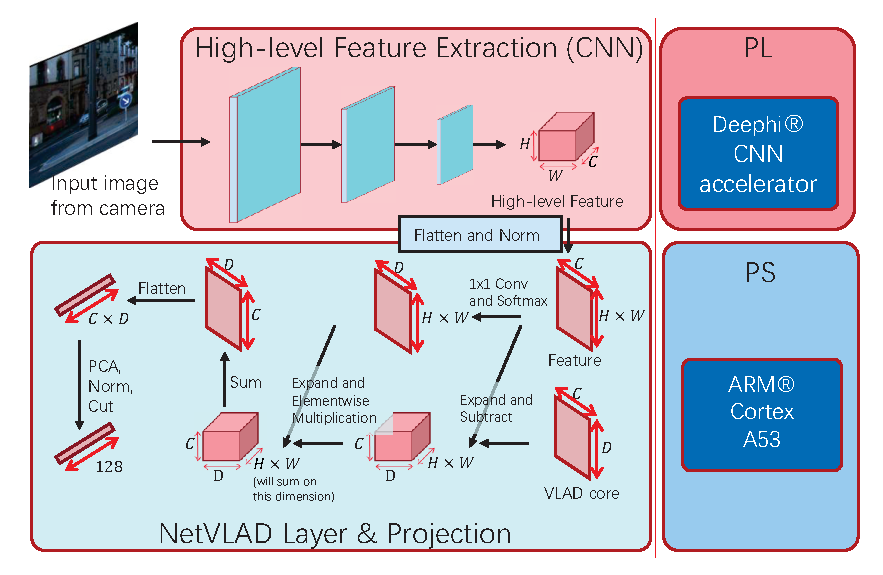
\includegraphics[width=0.95\linewidth]{fig/NetVLAD.eps}
%     \caption{Process of NetVLAD. The CNN encoder is running at the CNN acclerator on PL side, and the VLAD layer as well as the PCA is running at the ARM core at PS side.}
%     \label{fig:NetVLAD}
% \end{figure}

The place recognition method provide the encoded vector transferred to the central agent for inter-robot place matching. As described in \cref{sec:background}, CNN has achieved significant improvements in place recognition tasks, and NetVLAD \cite{Arandjelovic:2017997} is one of the most impressive methods. The CNN-based place recognition methods give the global descriptor of a camera frame in a two-step manner: $1)$ Firstly, a CNN encoder fetches the high-level feature map. $2)$ A vectorization component that aggregates the feature map into a shot global descriptor. The VLAD layer \cite{Arandjelovic:2017997} is a recently proposed plug-and-play operation that greatly improves the performance of place recognition. In the original work with the VLAD layer \cite{Arandjelovic:2017997}, the feature extraction encoder is a typical CNN named VGG-16 \cite{Simonyan:20143be}. The output dimension of original NetVLAD is usually tens of thousands, which is very difficult to be stored on the embedded system, not to mention in the communication-constrained environment. The PCA and the projection method can drastically reduce the output dimension. The previous works\cite{Cieslewski:20187ee} show that 128 dimension is plenty for DSLAM. The data flow and operations of the NetVLAD layer and the projection are complex and require the floating-point number, which cannot be supported with Deephi DPU. We implement the NetVLAD layer and the projection on the PS side of Zynq MPSoC.


Unlike the fixed-point finetune method used for pose estimation. The training procedure with huge non-public datasets is very complicated, and also we cannot finetune the NetVLAD model because of the lack of training data. We simply analyze the dynamic range of the weight and intermediate feature map of each CNN layer and figure out the optimal decimal point position for each layer respectively to minimize the truncation error of each layer.
This method is proposed in \cite{Qiu:2016151} and is used in many tasks such as image classification and image detection.

\subsection{Parallel Scheduling for VO and NetVLAD}

The time consumption of NetVLAD and VO is imbalanced. We do pipeline optimization to schedule the two components on Zynq MPSoC efficiently. The pipeline is illustrated in \cref{fig:pipline}. The interval time for reading camera is $T_{f}$. The CNN time for NetVLAD and VO is $T_{0}$ and $T_{1}$. The computation time cost on PS for VO and NetVLAD is $T_{2}$ and $T_{3}$. We do VO every input frame and do NetVLAD every $N$ frames.

\begin{figure}[t]
    \centering  
    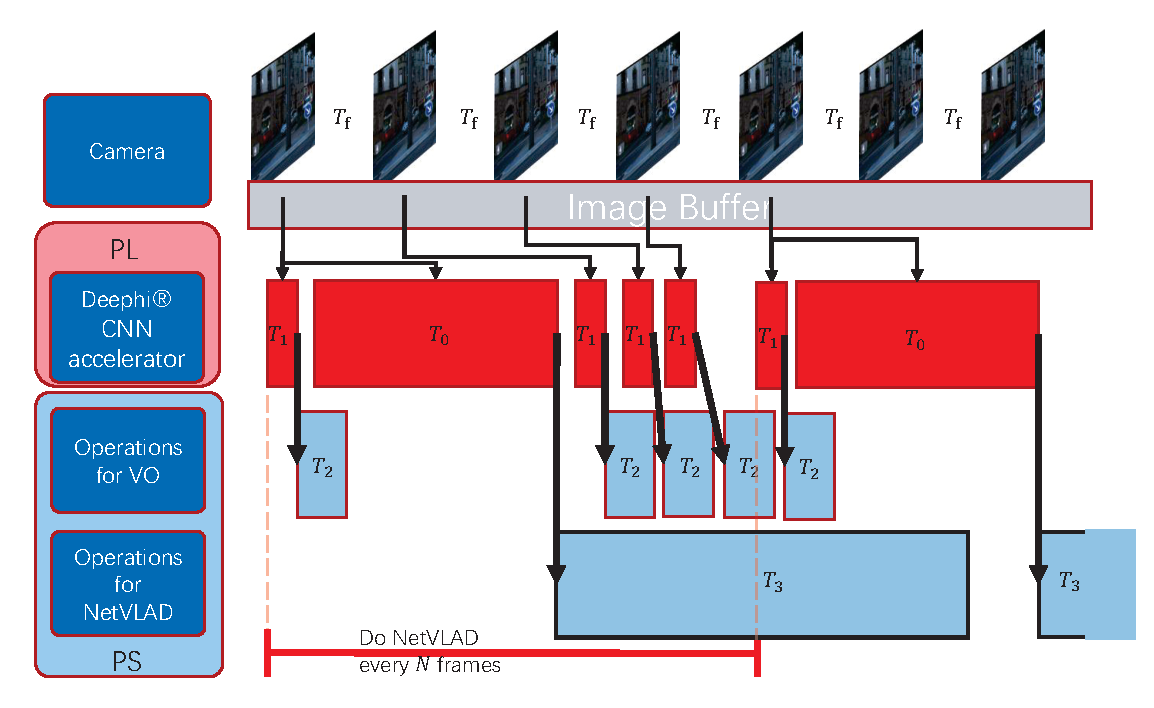
\includegraphics[width=0.95\linewidth]{fig/pipeline.eps}
    \caption{Scheduling pipeline. There are four threads: Camera read, Deephi core at PL, PS Operations for VO, and PS Operations for NetVLAD.}
    \label{fig:pipline}
\end{figure}

% The constrain of these computation time and $N$ is given as \cref{equ:pipline}.

Considering the thread on PL, the time constraint is given as \cref{equ:pipeline1}. 

\begin{equation}
    N \times T_{f} > T_{0} + N \times T_{1}
    \label{equ:pipeline1}
\end{equation}

The thread for VO on PS constrains the NetVLAD frequency as \cref{equ:pipeline2}.

\begin{equation}
    N \times T_{f} > T_{0} + T_{1} + (N-1) \times T_{2}
    \label{equ:pipeline2}
\end{equation}

The PS part of NetVLAD should finish before computing the PS part of next NetVLAD frame. This constraint can be written as \cref{equ:pipeline3}.

% The PS part of NetVLAD should finish before computing the PS part for next NetVLAD frame, and can be writen as \cref{equ:pipline3}.

\begin{equation}
    N \times T_{f} > T_{3}
    \label{equ:pipeline3}
\end{equation}

The execution time of our design will be given in \cref{sec:experiment}.


\section{Experiments}
\label{sec:experiment}
The speed and the accuracy of our proposed hardware-software co-design DSLAM will be evaluated in this section.

\subsection{Run-Time}

We evaluate our DSLAM on two intelligent cars which are controlled by the Deephi Aristotle board with a ZU9 MPSOC. The intelligent car and the board is illustrated in \cref{fig:env}. \Cref{tab:time} shows the run time of each part of our DSLAM system. The pipeline of scheduling of these parts is shown in \cref{sec:background}.


\begin{figure}[t]
    \centering  
    \includegraphics[width=0.95\linewidth]{fig/env.eps}
    \caption{The intelligent car with the Zynq MPSoC board.}
    \label{fig:env}
\end{figure}

\begin{table}[h]
    \centering
    \caption{Run-Time of each part in our DSLAM}
    \footnotesize
    \begin{threeparttable}
  % Table generated by Excel2LaTeX from sheet 'Sheet2'
  \setlength{\tabcolsep}{1mm}{
% Table generated by Excel2LaTeX from sheet 'Sheet1'
    \begin{tabular}{|c|c|c|c|c|}
    \hline
          & NetVLAD, PL & VO, PL  & VO, PS  & NetVLAD, PS  \bigstrut[t]\\
          & ($T_{0}$) &  ($T_{1}$) &  ($T_{2}$) &  ($T_{3}$) \bigstrut[b]\\
    \hline
    Execute time & \multirow{2}[2]{*}{66} & \multirow{2}[2]{*}{3} & \multirow{2}[2]{*}{10} & \multirow{2}[2]{*}{354} \bigstrut[t]\\
    (ms)  &       &       &       &  \bigstrut[b]\\
    \hline
    \end{tabular}%
    
  }
  \begin{tablenotes}
        \item[*] We read the camera at 20fps, so the $T_{f}$ in \cref{fig:pipline} is 50ms.
        \end{tablenotes}
      \end{threeparttable}
    \label{tab:time}%
    
  \end{table}%

Substituting the run-time of each part into \cref{equ:pipeline1,equ:pipeline2,equ:pipeline3}. We find out that the run-time of NetVLAD on PS ($T_{3}$) becomes the bottleneck of the system and \cref{equ:pipeline3} constrains the NetVLAD frequency ($N$) to $8$.

We calculate the relative 6-D pose between every two successive frames and the NetVLAD code every $8$ frames in the following experiments.

\subsection{VO with DPU}

We evaluate our VO approach with DPU on KITTI dataset \cite{geiger2013vision}. The dataset contains 11 labeled video sequences with stereo pairs, with original image size at $1242 \times 375$ pixels. In our design, we resize the image to $608 \times 160$ as the original Deepth-VO-Feate does \cite{Zhan:2018e92}.

% FIXME: 下面给了09和10的结果,这里finetune使用的数据集是不是需要修改一下
At the fixed-finetune procedure, we use the stereo pairs in sequences 01 to 10 as the training set. The training super parameters in \cref{equ:loss} are $[\lambda_{ir},\lambda_{fr},\lambda_{ds}] = [1,0.1,10]$. At the evaluation procedure, we use the left-eye input images of the stereo pairs of the 00 sequence of KITTI as the test set.

\begin{table}[ht]
    \centering
    \caption{Visual odometry (VO) results on test sequences (09, 10)}
    \footnotesize
    \begin{threeparttable}
\begin{tabular}{|c||cc|cc|c|}
  \hline
  \multirow{2}[2]{*}{method} & \multicolumn{2}{c|}{Seq. 09} & \multicolumn{2}{c|}{Seq. 10} & run time  \bigstrut[t]\\
                             & $t_{err}$        & $r_{err}$ & $t_{err}$        & $r_{err}$ & $(ms/frame)$ \bigstrut[b]\\
  \hline
  ORB-SLAM  &15.30 &0.26 &3.68 &0.48 &  \bigstrut\\
  \hline
  Ours(float)  &10.49 &3.34 &11.64 &3.14 &  \bigstrut\\
  \hline
  Ours(fixed)  &10.27 &4.08 &8.84 &4.01 & 12 \bigstrut\\
  \hline
  \end{tabular}
  
  \begin{tablenotes}
        \item[*] $t_{err}(\%)$ is the average translational drift error. $r_{err}({}^{\circ}/100m)$ is average rotational drift error.
        \end{tablenotes}
      \end{threeparttable}
    \label{tab:VO}%
  \end{table}%

  % FIXME: 给出的是09和10的结果
  % We evaluate the VO on the sub-sequences at length of ??? and report the average translational and rotational errors for the testing sequence 00 in \cref{tab:VO}.  The comparison of the estimated trajectory for the methods is illustrated in \cref{fig:VO}.
  We evaluate the Viusal Odometry on KITTI odometry dataset and report the average translational and rotational errors for the testing sequences 09 and 10 in \cref{tab:VO}.  The comparison of the estimated trajectory for the methods is illustrated in \cref{fig:VO}.


  \begin{figure}[t]
    \centering  
    \subfigure[Traj. on Seq. 09] {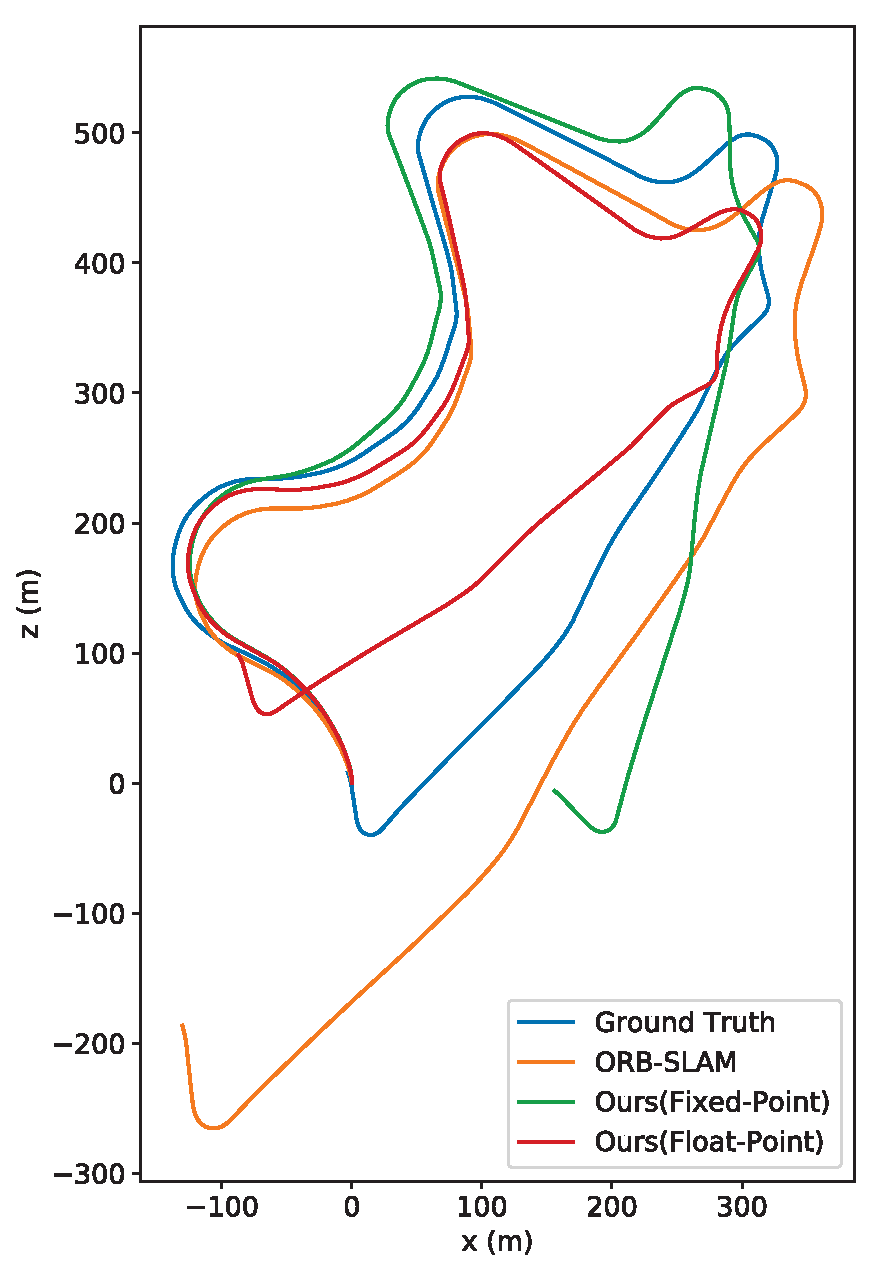
\includegraphics[height=0.9\linewidth]{fig/sequence_09.eps}} 
    \subfigure[Traj. on Seq. 10] {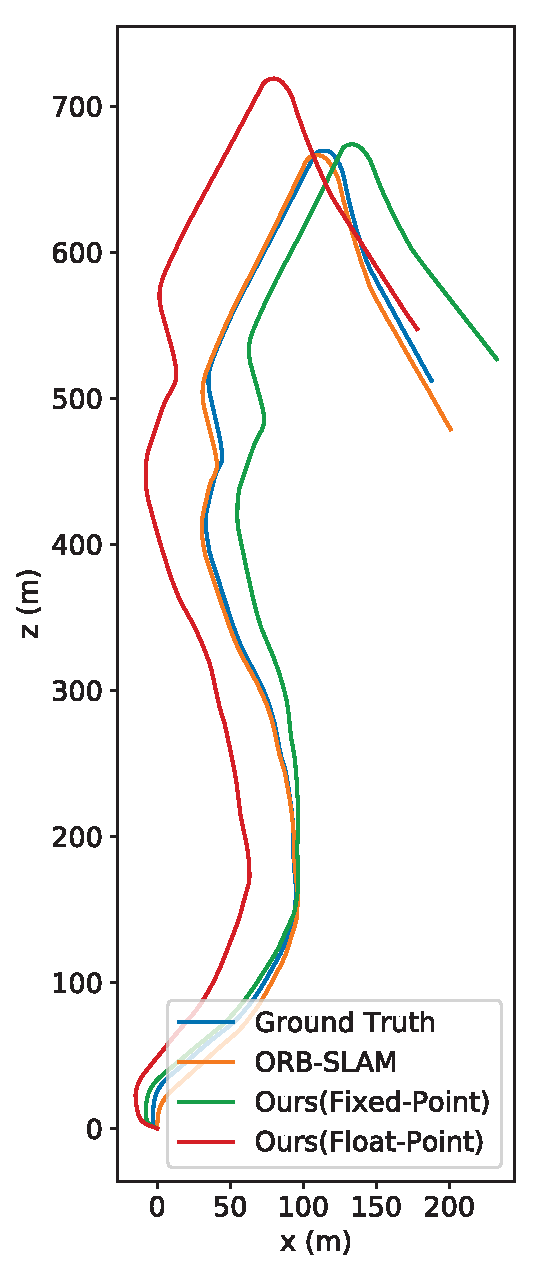
\includegraphics[height=0.9\linewidth]{fig/sequence_10.eps}} 
    \caption{Qualitative evaluation of odometry on the KITTI Odometry test sequences (09, 10).}
    \label{fig:VO}
  \end{figure}


Because of the fixed-point number used in our design, which sacrifices the precision of the CNN, the VO accuracy is not as good as the previous works \cite{Mur-Artal:2017281, Zhan:2018e92}. On the other hand, our VO can calculate the 6-D pose within $20ms$ on a resource-constrained embedded platform.

\subsection{NetVLAD with DPU}

We evaluate the NetVLAD performance on the loop close dataset for KITTI\cite{KITTIGroundTruth}.
The dataset labels the ground truth of loop closure for these sequences based on the metric positions of each image. Specifically, it compares the position of each image to the others in the sequence and regards the one as a loop if it lies within a radius of $6m$.

The precision-recall curves of the original NetVLAD with an output of 4096 dimensions (Blue), fixed-point NetVLAD 4096-D output (Green), original NetVLAD with 128-D output (Red), and fixed-point NetVLAD 128-D output (Yellow) are shown in \cref{fig:reloc}. We use sequence 00 as the test sequence.


\begin{figure}[t]
  \centering  
  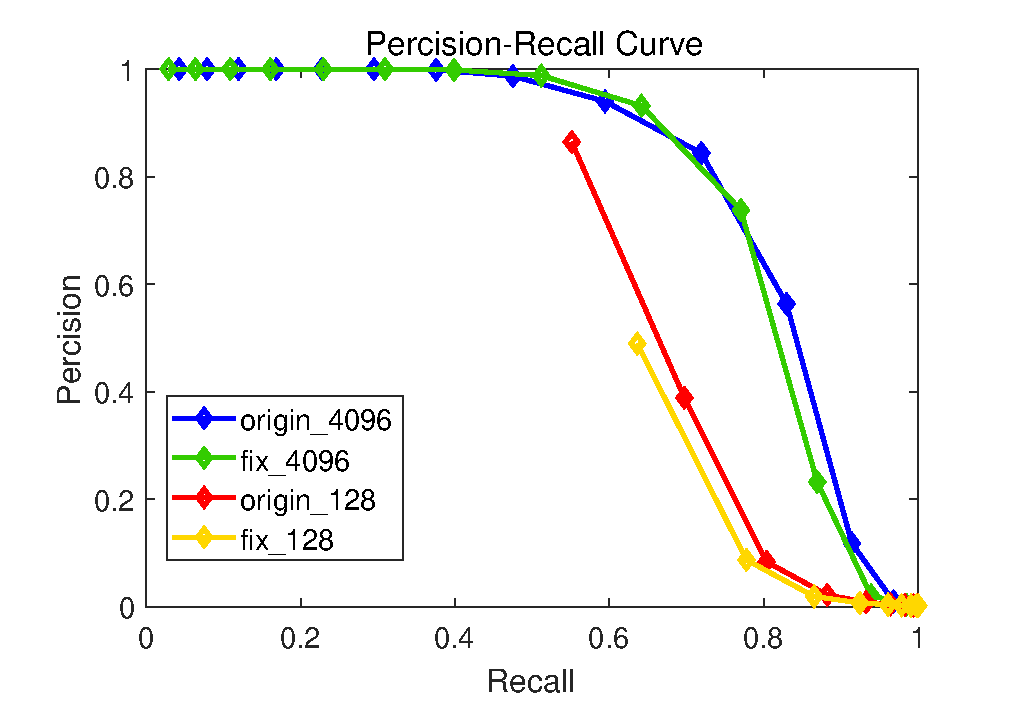
\includegraphics[width=0.85\linewidth]{fig/val_reloc.eps}
  \caption{ROC curves on sequence 00.}
  \label{fig:reloc}
\end{figure}

Our NetVLAD with DPU performs similarly to the original NetVLAD with the same output dimension but runs much faster with the help of the acceleration techniques on FPGA and architecture design. Even if there are sightly accuracy reduction on the ROC curves, the following experiment shows that the slight drawback would not make the overall DSLAM performance decline.

\subsection{DSLAM Evaluation}

With the help of our hardware-software co-design VO and place recognition components on the embedded system, we can build up the DSLAM system like the previous work \cite{Cieslewski:20187ee}. However, unlike the feature point based method in previous \cite{Cieslewski:20187ee}, our approach does not necessarily compute the feature point for each frame. The previous work \cite{Cieslewski:20187ee} transfers the ORB feature points among agents to do inter-robot pose estimation and trajectory merging.

%讲下更具体的实验设计

A possible way to solve the inter-robot pose estimation is to calculate the feature points and descriptors of the corresponding robot and frames when the inter-robot loop closure occurs. However, on the one hand, the traditional feature point detection and description method cannot get the absolute scale from a single image. On the other hand, it is resource consuming to do feature point algorithms like SIFT\cite{Jegou:2010f45} and ORB\cite{Mur-Artal:2017281}. The agents may stop and solve the feature points. We directly transfer the down-sampled $608 \times 160$ image among the agents and use the same method as the proposed VO with DPU to do the inter-robot pose estimation. The result of the merged trajectory is illustrated in \cref{fig:dslam}.


\begin{figure}[ht]
  \centering  
  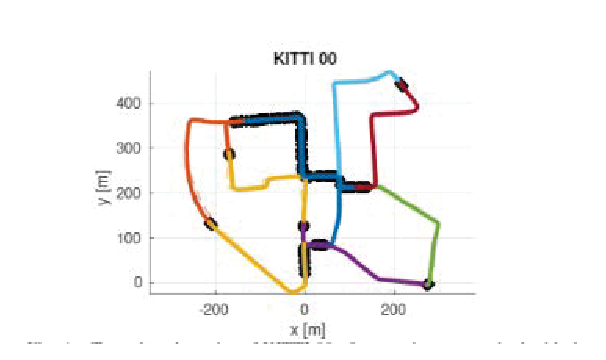
\includegraphics[width=0.85\linewidth]{fig/dslam.eps}
  \caption{??? The sub-trajectory of each agent and the merged trajectory.}
  \label{fig:dslam}
\end{figure}

\begin{figure}[thb]
  \centering  
  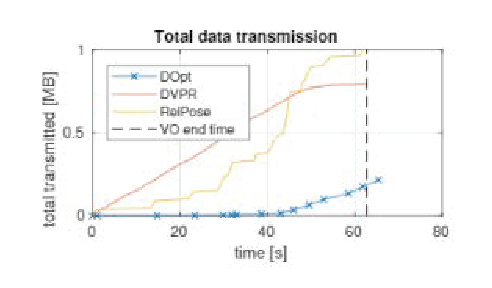
\includegraphics[width=0.85\linewidth]{fig/data.eps}
  \caption{??? The total communication traffic of the propsoed DSLAM}
  \label{fig:data}
\end{figure}

There are three kinds of data need to be transferred among the agents and the server: $1)$ the VO results of each frame (VO), $2)$ the NetVLAD results of every $8$ frames (NetVLAD), $3)$ the image need for inter-robot relative pose estimation (RelPose).

At the beginning of the task, there is no inter-robot loop closure detected, so there is no data traffic for RelPose. When inter-robot loop closure occurs, the data traffic for RelPose increases rapidly. The previous work\cite{Cieslewski:20187ee} also faces this problem though it uses feature point for inter-robot relative pose estimation.


The total communication traffic of the proposed DSLAM system on KITTI 00 is increasing with time and is shown in \cref{fig:data}.


\section{Conclusion}
\label{sec:conclusion} 

We propose a hardware-software co-design DSLAM system with the help of Xilinx Zynq MPSoC and Deephi DPU. We optimize two essential components of DSLAM system,  1)Visual Odometry(VO) and 2) Place Recognition on the embedded system. From the aspect of calculation, the vectorization and projection operations on the PS side of Zynq MPSoC needed by NetVLAD is the bottleneck to do more frequent place recognition. From the aspect of communication, the data traffic for inter-robot relative pose estimation consumes the most communication resources. The accelerator for vectorization based on FPGA and more data-efficient inter-robot pose estimation method could be researched in future work.


\section*{Acknowledgment}
This work was supported by National Natural Science Foundation of China (Grant No.61874156)


\bibliographystyle{IEEEtran}
\bibliography{src/fpgaslam}

\end{document}
